% Options for packages loaded elsewhere
% Options for packages loaded elsewhere
\PassOptionsToPackage{unicode}{hyperref}
\PassOptionsToPackage{hyphens}{url}
\PassOptionsToPackage{dvipsnames,svgnames,x11names}{xcolor}
%
\documentclass[
  letterpaper,
  DIV=11,
  numbers=noendperiod]{scrartcl}
\usepackage{xcolor}
\usepackage{amsmath,amssymb}
\setcounter{secnumdepth}{-\maxdimen} % remove section numbering
\usepackage{iftex}
\ifPDFTeX
  \usepackage[T1]{fontenc}
  \usepackage[utf8]{inputenc}
  \usepackage{textcomp} % provide euro and other symbols
\else % if luatex or xetex
  \usepackage{unicode-math} % this also loads fontspec
  \defaultfontfeatures{Scale=MatchLowercase}
  \defaultfontfeatures[\rmfamily]{Ligatures=TeX,Scale=1}
\fi
\usepackage{lmodern}
\ifPDFTeX\else
  % xetex/luatex font selection
\fi
% Use upquote if available, for straight quotes in verbatim environments
\IfFileExists{upquote.sty}{\usepackage{upquote}}{}
\IfFileExists{microtype.sty}{% use microtype if available
  \usepackage[]{microtype}
  \UseMicrotypeSet[protrusion]{basicmath} % disable protrusion for tt fonts
}{}
\makeatletter
\@ifundefined{KOMAClassName}{% if non-KOMA class
  \IfFileExists{parskip.sty}{%
    \usepackage{parskip}
  }{% else
    \setlength{\parindent}{0pt}
    \setlength{\parskip}{6pt plus 2pt minus 1pt}}
}{% if KOMA class
  \KOMAoptions{parskip=half}}
\makeatother
% Make \paragraph and \subparagraph free-standing
\makeatletter
\ifx\paragraph\undefined\else
  \let\oldparagraph\paragraph
  \renewcommand{\paragraph}{
    \@ifstar
      \xxxParagraphStar
      \xxxParagraphNoStar
  }
  \newcommand{\xxxParagraphStar}[1]{\oldparagraph*{#1}\mbox{}}
  \newcommand{\xxxParagraphNoStar}[1]{\oldparagraph{#1}\mbox{}}
\fi
\ifx\subparagraph\undefined\else
  \let\oldsubparagraph\subparagraph
  \renewcommand{\subparagraph}{
    \@ifstar
      \xxxSubParagraphStar
      \xxxSubParagraphNoStar
  }
  \newcommand{\xxxSubParagraphStar}[1]{\oldsubparagraph*{#1}\mbox{}}
  \newcommand{\xxxSubParagraphNoStar}[1]{\oldsubparagraph{#1}\mbox{}}
\fi
\makeatother


\usepackage{longtable,booktabs,array}
\newcounter{none} % for unnumbered tables
\usepackage{calc} % for calculating minipage widths
% Correct order of tables after \paragraph or \subparagraph
\usepackage{etoolbox}
\makeatletter
\patchcmd\longtable{\par}{\if@noskipsec\mbox{}\fi\par}{}{}
\makeatother
% Allow footnotes in longtable head/foot
\IfFileExists{footnotehyper.sty}{\usepackage{footnotehyper}}{\usepackage{footnote}}
\makesavenoteenv{longtable}
\usepackage{graphicx}
\makeatletter
\newsavebox\pandoc@box
\newcommand*\pandocbounded[1]{% scales image to fit in text height/width
  \sbox\pandoc@box{#1}%
  \Gscale@div\@tempa{\textheight}{\dimexpr\ht\pandoc@box+\dp\pandoc@box\relax}%
  \Gscale@div\@tempb{\linewidth}{\wd\pandoc@box}%
  \ifdim\@tempb\p@<\@tempa\p@\let\@tempa\@tempb\fi% select the smaller of both
  \ifdim\@tempa\p@<\p@\scalebox{\@tempa}{\usebox\pandoc@box}%
  \else\usebox{\pandoc@box}%
  \fi%
}
% Set default figure placement to htbp
\def\fps@figure{htbp}
\makeatother





\setlength{\emergencystretch}{3em} % prevent overfull lines

\providecommand{\tightlist}{%
  \setlength{\itemsep}{0pt}\setlength{\parskip}{0pt}}



 


\KOMAoption{captions}{tableheading}
\makeatletter
\@ifpackageloaded{tcolorbox}{}{\usepackage[skins,breakable]{tcolorbox}}
\@ifpackageloaded{fontawesome5}{}{\usepackage{fontawesome5}}
\definecolor{quarto-callout-color}{HTML}{909090}
\definecolor{quarto-callout-note-color}{HTML}{0758E5}
\definecolor{quarto-callout-important-color}{HTML}{CC1914}
\definecolor{quarto-callout-warning-color}{HTML}{EB9113}
\definecolor{quarto-callout-tip-color}{HTML}{00A047}
\definecolor{quarto-callout-caution-color}{HTML}{FC5300}
\definecolor{quarto-callout-color-frame}{HTML}{acacac}
\definecolor{quarto-callout-note-color-frame}{HTML}{4582ec}
\definecolor{quarto-callout-important-color-frame}{HTML}{d9534f}
\definecolor{quarto-callout-warning-color-frame}{HTML}{f0ad4e}
\definecolor{quarto-callout-tip-color-frame}{HTML}{02b875}
\definecolor{quarto-callout-caution-color-frame}{HTML}{fd7e14}
\makeatother
\makeatletter
\@ifpackageloaded{caption}{}{\usepackage{caption}}
\AtBeginDocument{%
\ifdefined\contentsname
  \renewcommand*\contentsname{Table of contents}
\else
  \newcommand\contentsname{Table of contents}
\fi
\ifdefined\listfigurename
  \renewcommand*\listfigurename{List of Figures}
\else
  \newcommand\listfigurename{List of Figures}
\fi
\ifdefined\listtablename
  \renewcommand*\listtablename{List of Tables}
\else
  \newcommand\listtablename{List of Tables}
\fi
\ifdefined\figurename
  \renewcommand*\figurename{Figure}
\else
  \newcommand\figurename{Figure}
\fi
\ifdefined\tablename
  \renewcommand*\tablename{Table}
\else
  \newcommand\tablename{Table}
\fi
}
\@ifpackageloaded{float}{}{\usepackage{float}}
\floatstyle{ruled}
\@ifundefined{c@chapter}{\newfloat{codelisting}{h}{lop}}{\newfloat{codelisting}{h}{lop}[chapter]}
\floatname{codelisting}{Listing}
\newcommand*\listoflistings{\listof{codelisting}{List of Listings}}
\makeatother
\makeatletter
\makeatother
\makeatletter
\@ifpackageloaded{caption}{}{\usepackage{caption}}
\@ifpackageloaded{subcaption}{}{\usepackage{subcaption}}
\makeatother
\usepackage{bookmark}
\IfFileExists{xurl.sty}{\usepackage{xurl}}{} % add URL line breaks if available
\urlstyle{same}
\hypersetup{
  pdftitle={Analyses at the Census Tract},
  pdfauthor={Cal-Adapt Analytics Engine Team},
  colorlinks=true,
  linkcolor={blue},
  filecolor={Maroon},
  citecolor={Blue},
  urlcolor={Blue},
  pdfcreator={LaTeX via pandoc}}


\title{Analyses at the Census Tract}
\author{Cal-Adapt Analytics Engine Team}
\date{2026-06-02}
\begin{document}
\maketitle


Many planners, agencies, and community organizations use census tract
data because it can enable targeted planning, policy, and programmatic
decision making at a local level. It is therefore common for
practitioners to ask whether climate model projections can be translated
to census tracts to support their analyses, particularly those that may
require overlays with demographic information. However, climate models
do not produce data at census tract resolution. This introduces
important risks and limitations when attempting to map gridded climate
data onto these boundaries.

\subsection{Analytics Engine Support for Census Tract
Analysis}\label{analytics-engine-support-for-census-tract-analysis}

To support needs for climate data at a census tract level, the Analytics
Engine (AE) team has developed a Python-based tool called \texttt{clip}
within the project's
\href{https://github.com/cal-adapt/climakitae}{climakitae} Python
toolkit that allows users to clip gridded climate datasets to census
tract polygons. For more details on how to use this \texttt{clip} tool
with \texttt{"clip":\ "\textless{}geoid\textgreater{}"} or
\texttt{"clip:\ {[}"\textless{}geoid\textgreater{}",\ …{]}}, please
navigate to the ``Processor Example 5: Clipping to Boundaries'' section
in the
\href{https://github.com/cal-adapt/cae-notebooks/blob/main/basic_data_access.ipynb}{Data
Access Notebook}.

The following guidance describes the key risks and technical challenges
associated with conducting census tract-level analyses with climate
data. It aims to provide guidance on which information census
tract-level estimates can and cannot reliably provide.

The Analytics Engine team's goal is not to deliver authoritative
``census tract climate datasets'', but to provide transparent,
reproducible tools that allow users to explore climate data responsibly.
The \emph{\href{https://github.com/cal-adapt/climakitae}{climakitae}}
census tract clipping tool is intended as a learning and analysis aid,
paired with guidance like this page to help users understand the
assumptions, risks, and appropriate interpretations involved in using
climate data at a census tract level.

\subsection{Census Tract Analyses Present Unique
Challenges}\label{census-tract-analyses-present-unique-challenges}

The climate models used in the Analytics Engine produce data on regular
grid cells of a fixed 3 x 3 kilometer size. US census tracts, by
contrast, are irregularly shaped statistical areas within a county whose
size varies widely depending on population density; they are generally
designed to represent 1,200 to 8,000 people
(\href{https://www.census.gov/programs-surveys/geography/about/glossary.html\#par_textimage_13}{U.S.
Census Bureau, 2022}). In population-dense areas like downtowns, census
tracts can be very small (such as a few city blocks), while in rural
areas, a single census tract can occupy a large portion of the county.
This difference in census tract size can make translating gridded data
onto a census tract-level tricky.

Climate models do not produce data at census tract resolution. Most
datasets used in the Analytics Engine are produced on
\href{https://climateestimate.net/content/gridded-data.html\#:~:text=Gridded\%20data\%20products\%20are\%20a\%20combination\%20of,the\%20entire\%20globe\%20or\%20a\%20specific\%20region.}{equal-area
grid cells} that are much larger than many urban census tracts, and much
smaller than rural area census tracts. This fundamental mismatch creates
several technical challenges that users should carefully consider:

\subsubsection{Spatial Mismatch and Grid-Scale
Representation}\label{spatial-mismatch-and-grid-scale-representation}

In dense urban areas, multiple census tracts may fall entirely within a
single model grid cell. In these cases, the same climate variable value
(e.g.~temperature) will be assigned to several census tracts, even
though real-world conditions may vary meaningfully across neighborhoods
due to the built environment, land cover, or proximity to water
(Figure~\ref{fig-sf-tracts}). For dynamically downscaled datasets such
as WRF, each grid cell value represents conditions at the grid cell's
center point and is assumed to be representative of the broader grid
area (3km x 3km). Sub-grid variability (such as sharp elevation changes,
coastal gradients, or urban features) is not explicitly resolved. As a
result, when census tracts are smaller than a grid cell, or intersect
only a portion of one, users should keep in mind that the climate value
reflects a modeled approximation rather than conditions everywhere
within that area. These tract-level differences are not resolved by the
climate model and should not be inferred from the data.

\begin{figure}

\centering{

\pandocbounded{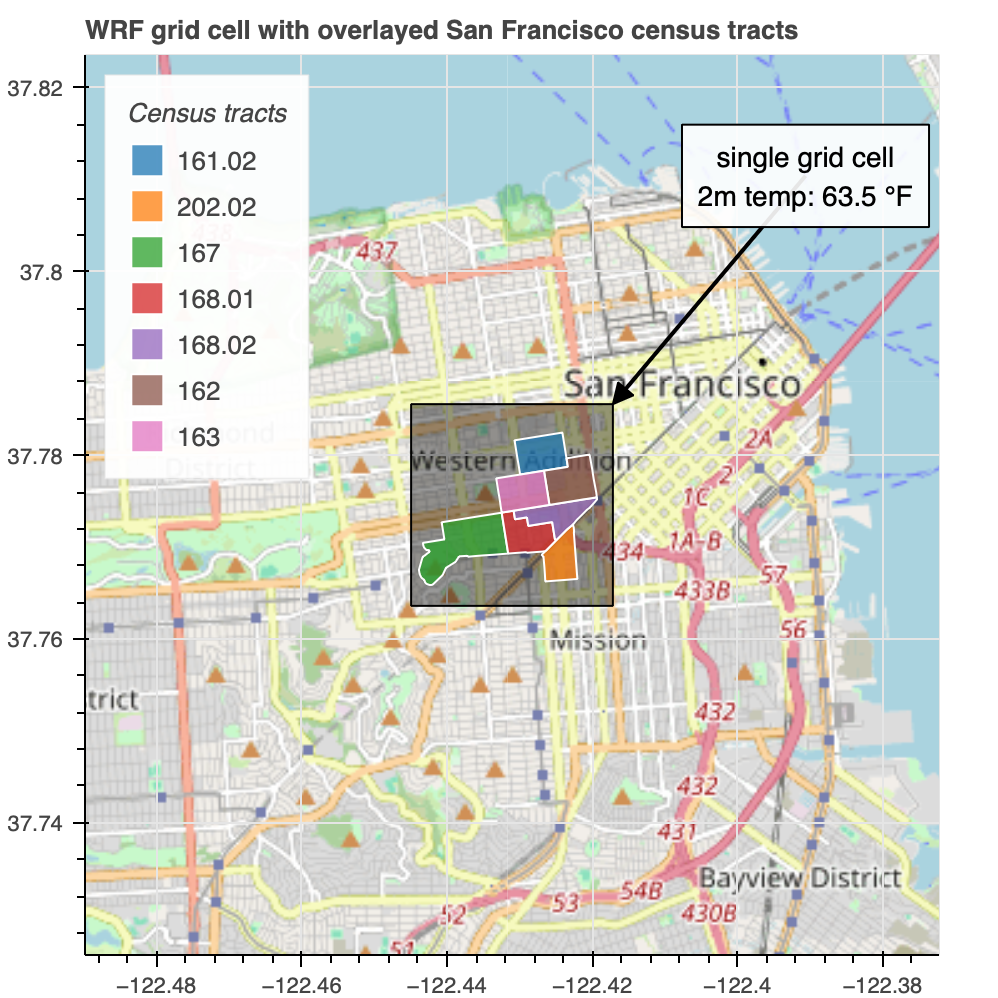
\includegraphics[keepaspectratio]{figures/static/census_tract_fig1.png}}

}

\caption{\label{fig-sf-tracts}Example of spatial mismatch between a
single model grid cell and multiple census tracts within the city of San
Francisco, CA. If extracting air temperature for these seven census
tracts, each tract would result in the same value, despite actual
microclimatic differences within these neighborhoods. Census tracts
shown here are: 161.02, 202.02, 167.00, 168.01, 168.02, 162.00, 163.00,
San Francisco, CA.}

\end{figure}%

\subsubsection{Aggregation Issues}\label{aggregation-issues}

Census tracts and grid cells are not a perfect one-to-one match. In
rural areas, a single census tract may span many grid cells that differ
substantially in elevation, land cover, or climate. Any value summarized
across the tract (such as a mean or percentile) will smooth this
variability. As a result, a tract-wide average may not be representative
of the conditions experienced by most locations within that tract
(Figure~\ref{fig-rural-tract}).

\begin{figure}

\centering{

\pandocbounded{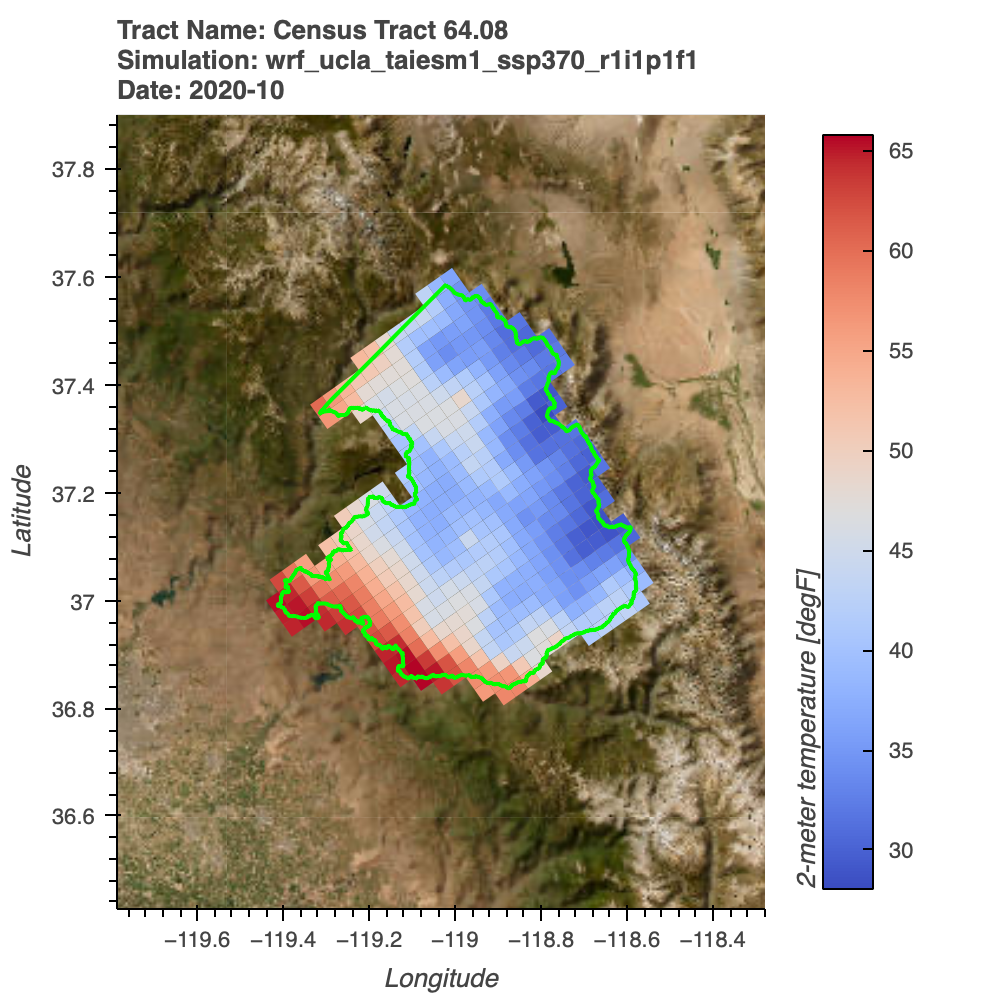
\includegraphics[keepaspectratio]{figures/static/census_tract_fig2.png}}

}

\caption{\label{fig-rural-tract}Example of a large rural census tract in
eastern Fresno County spanning Sierra Nevada foothills into higher
elevation terrain, covering multiple climate model grid cells. If
extracting a single representative air temperature value for this census
tract, the variability of temperatures would be substantially smoothed,
and may not accurately represent realistic conditions. The census tract
shown here is Census Tract 64.08, Fresno County, CA.}

\end{figure}%

\subsubsection{Coastal Census Tracts}\label{coastal-census-tracts}

In coastal areas, census tracts may intersect grid cells that are
partially or mostly over water. For example, the census tract that
houses the University of California Santa Barbara includes coastal and
off-shore grid cells, which have different temperature characteristics
than the adjacent land. When these grid cells are averaged at a census
tract level, the resulting values may appear cooler or less extreme than
the conditions actually experienced on land. While this issue is not
unique to census tracts and reflects a broader limitation of gridded
climate data over complex geography, it becomes an especially important
consideration when working with climate data at these small spatial
scales.

\subsubsection{Sub-Grid Variability}\label{sub-grid-variability}

For dynamically downscaled datasets such as WRF, each grid cell value
represents conditions at the grid cell's center point and is assumed to
be representative of the broader grid area (3km x 3km). Sub-grid
variability (such as sharp elevation changes, coastal gradients, or
urban features) is not explicitly resolved. When census tracts are
smaller than a grid cell, or intersect only a portion of one, users
should keep in mind that the climate value reflects a modeled
approximation rather than conditions everywhere within that area.

\begin{tcolorbox}[enhanced jigsaw, arc=.35mm, bottomrule=.15mm, bottomtitle=1mm, breakable, colback=white, colbacktitle=quarto-callout-note-color!10!white, colframe=quarto-callout-note-color-frame, coltitle=black, left=2mm, leftrule=.75mm, opacityback=0, opacitybacktitle=0.6, rightrule=.15mm, title=\textcolor{quarto-callout-note-color}{\faInfo}\hspace{0.5em}{Note}, titlerule=0mm, toprule=.15mm, toptitle=1mm]

Census tract boundaries change over time as populations shift and
definitions are updated. The Analytics Engine uses a specific census
tract vintage:
\href{https://catalog.data.gov/dataset/tiger-line-shapefile-2020-state-california-census-tracts}{TIGER/Line
Shapefile, 2020, State, California, Census Tracts}. Tract-based analyses
may not align perfectly with older or newer demographic datasets.

\end{tcolorbox}

Therefore, climate model data that is extracted at the census-tract
level should not be treated as representative climate values for that
tract. Rather, this data should be viewed as an approximation of the
climate, with uncertainty introduced by the size of the model grid and
how it represents real-world geography.

\subsection{Appropriate and Inappropriate
Analyses}\label{appropriate-and-inappropriate-analyses}

\subsubsection{Appropriate Analyses}\label{appropriate-analyses}

Using climate data at a census tract-level can be useful for certain
types of exploratory or screening-level analyses, particularly when the
goal is to understand broad spatial patterns rather than precise local
values. For example:

\begin{itemize}
\tightlist
\item
  When identifying general ``hotter'' or ``colder'' parts of a region to
  support high-level prioritization
  (\href{https://doi.org/10.1016/j.uclim.2023.101711}{Szagri et al.,
  2023}); e.g.~cooling demand may be higher for inland census tracts
  that are relatively warmer than nearby coastal tracts, even if exact
  temperatures cannot be resolved at the neighborhood scale.
\item
  Overlaying climate indicators with demographic or vulnerability
  datasets to understand regional patterns or disparities
  (\href{https://doi.org/10.1016/j.mex.2025.103290}{McCullagh et al.,
  2025}); e.g.~identifying census tracts with both higher projected
  extreme heat exposure and higher proportions of elderly residents to
  flag areas where heat-related health risks may be elevated at a
  regional scale, without interpreting the values as
  precise-neighborhood-level temperatures.
\item
  Supporting qualitative or comparative assessments where relative
  differences matter more than precise magnitudes; e.g.~comparing
  whether one group of census tracts is generally warmer or experiences
  more extreme heat days than another group (such as inland versus
  coastal tracts) to inform discussion, screening, or prioritization
  (rather than to calculate exact thresholds or design specifications).
\end{itemize}

In these contexts, tract-level climate estimates can help frame
questions and guide further analysis, provided their limitations are
clearly acknowledged.

\subsubsection{Inappropriate Analyses}\label{inappropriate-analyses}

A census tract approach is generally not appropriate when:

\begin{itemize}
\tightlist
\item
  The decision requires accurate representation of neighborhood-scale
  temperatures, extremes, or microclimates
  (\href{https://doi.org/10.1175/BAMS-D-24-0230.1}{Fuhrmann et al.,
  2024}).
\item
  Results will be interpreted as precise predictions for a specific
  tract, for example, counting the number of days above a critical
  threshold.
\item
  The analysis depends on values that change significantly within
  individual grid cells (for example, coastal versus inland
  differences).
\item
  Infrastructure, sizing, or engineering decisions that require
  higher-resolution information than climate models can reliably
  provide.
\end{itemize}

\section{References}\label{references}

\begin{itemize}
\tightlist
\item
  Szagri, D., Nagy, B., \& Szalay, Z. (2023). How can we predict where
  heatwaves will have an impact? -- A literature review on heat
  vulnerability indexes. \emph{Urban Climate}, 52.
  \url{https://doi.org/10.1016/j.uclim.2023.101711}
\item
  McCullagh, D., Cámaro-García, W., Dunne, D., Nowbakht, P., Cumiskey,
  L., Gannon, C., \& Phillips, C. (2025). Development of a social
  vulnerability index: Enhancing approaches to support climate justice.
  \emph{MethodsX}, 14. \url{https://doi.org/10.1016/j.mex.2025.103290}
\item
  Fuhrmann, C., Robinson, A., Konrad, C., \& Bhatia, A. (2024). From
  Data to Action: How Urban Heat Mapping Campaigns Can Expose
  Vulnerabilities and Inform Local Heat Policy. \emph{Bulletin of the
  American Meteorological Society}, 105(11), E2078--E2084.
  \url{https://doi.org/10.1175/BAMS-D-24-0230.1}
\item
  U.S. Census Bureau. (2022). Census Tracts.
  \url{https://www.census.gov/programs-surveys/geography/about/glossary.html\#par_textimage_13}
\end{itemize}




\end{document}
